\section{采集函数}
\label{sec:bo-acquisition}

后验告诉了我们每个候选点上函数值的分布，但它没有说下一次该评价哪里。接下来要弄清：怎样把后验转成一个可以比较大小的分数？这个分数称为\term{采集函数}（acquisition function），记作$\alpha_t(\bm{x})$，下一个评价点取使它最大的位置。

好的分数要处理一对矛盾。后验均值低的地方看起来有希望，这是\emph{利用}；后验方差大的地方我们知之甚少，那里可能藏着好东西，这是\emph{探索}。各种采集函数的差别就在于用什么方式把两者结合起来。

本节先假定观测无噪声，当前已观测的最好值就是
\begin{equation}
 b_t=\min_{i\leq t}f(\bm{x}_i).
 \label{eq:bo-incumbent}
\end{equation}
下面统一按最小化比较。例子都用$t=3$时贯穿例的后验，$b_3=-0.3$，取整数候选点。

\subsection{改进概率（PI）}
\label{sec:bo-pi}

最朴素的想法是问：在这个位置评价，有多大可能比现在最好的结果更好？再要求至少好出一个幅度$\xi\geq0$，得到\term{改进概率}（probability of improvement，PI）：
\begin{equation}
 \mathrm{PI}_t(\bm{x})=\mathbb{P}\bigl(F(\bm{x})<b_t-\xi\mid\mathcal{D}_t\bigr)
 =\Phi\left(\frac{b_t-\xi-m_t(\bm{x})}{s_t(\bm{x})}\right),
 \label{eq:bo-pi}
\end{equation}
其中$s_t(\bm{x})>0$，$\Phi$是标准正态分布函数。$s_t(\bm{x})=0$时，函数值已确定，$\mathrm{PI}$依$m_t(\bm{x})<b_t-\xi$是否成立取$1$或$0$。

PI只数“是否过线”，不问过线之后好多少。比较两个候选，取$b_t=0$，$\xi=0$，
\[
 \text{A}:\ F\sim N(-0.1,\ 0.1^2),\qquad
 \text{B}:\ F\sim N(0.5,\ 1).
\]
代入式~\eqref{eq:bo-pi}，
\[
 \mathrm{PI}(\text{A})=\Phi(1)\approx0.841,\qquad
 \mathrm{PI}(\text{B})=\Phi(-0.5)\approx0.309.
\]
PI选A。图~\ref{fig:bo-pi-vs-ei}的绿色面积就是这两个概率。可是A即使成功也只改善零点几，B虽不常成功，一旦成功可能改善很多。

\begin{BookInlineFigure}
 \centering
 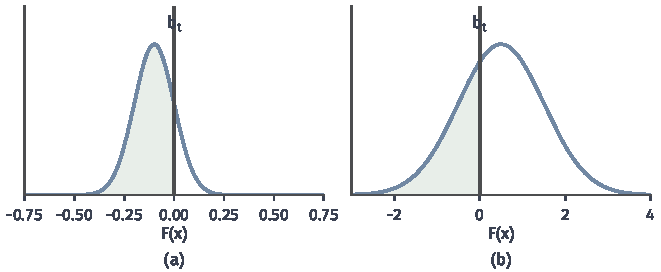
\includegraphics[width=112mm]{figures/05-optimization/05-stochastic-optimization/matplotlib/bo-pi-vs-ei/figure.pdf}
 \caption{改进的概率与幅度。蓝线是候选点函数值的后验密度，深灰竖线是当前最好值$b_t=0$，浅绿面积是改进概率。(a)候选A：$N(-0.1,0.1^2)$，大概率过线，但过线幅度很小。(b)候选B：$N(0.5,1)$，概率较小，但左尾可以伸得很远。两图横轴比例不同。}
 \label{fig:bo-pi-vs-ei}
\end{BookInlineFigure}

$\xi$的作用可以这样看。$\xi=0$时，紧贴着当前最好点的位置，后验均值几乎等于$b_t$，方差几乎为零，PI接近$1/2$，后面的图中可以看到，PI的最大点恰好贴在已观测的最好点旁边，这样的评价几乎不提供新信息。取$\xi>0$把门槛压低，这种贴边的小改进就不算数了。可是$\xi$取多大没有普适答案，它取决于函数值的尺度。

\subsection{期望改进（EI）}
\label{sec:bo-ei}

PI的缺陷指明了修改方向：把幅度也算进去。若在$\bm{x}$评价，新的最好值相比$b_t$的改善量是
\[
 \bigl(b_t-F(\bm{x})\bigr)_+=\max\{b_t-F(\bm{x}),0\}.
\]
没有改善时计为$0$，因为最好值不会变差。这个改善量的后验期望称为\term{期望改进}（expected improvement，EI）：
\begin{equation}
 \mathrm{EI}_t(\bm{x})=\mathbb{E}\bigl[(b_t-F(\bm{x}))_+\mid\mathcal{D}_t\bigr].
 \label{eq:bo-ei-def}
\end{equation}

\begin{theorem}[期望改进的闭式]
\label{thm:bo-ei}
设$F(\bm{x})\mid\mathcal{D}_t\sim N(m,s^2)$。若$s>0$，记$z=(b_t-m)/s$，则
\begin{equation}
 \mathrm{EI}_t(\bm{x})=(b_t-m)\Phi(z)+s\phi(z),
 \label{eq:bo-ei}
\end{equation}
其中$\Phi$、$\phi$分别是标准正态分布函数和密度函数。若$s=0$，则
\begin{equation}
 \mathrm{EI}_t(\bm{x})=(b_t-m)_+.
 \label{eq:bo-ei-zero}
\end{equation}
\end{theorem}

\begin{proof}
$s=0$时$F(\bm{x})=m$是确定的数，改善量就是$(b_t-m)_+$。

设$s>0$，把$F(\bm{x})$写成$m+sW$，$W\sim N(0,1)$，则
\[
 b_t-F(\bm{x})=s(z-W).
\]
所以
\[
 \mathrm{EI}_t(\bm{x})=s\int_{-\infty}^{z}(z-w)\phi(w)\,\mathrm{d}w
 =sz\Phi(z)-s\int_{-\infty}^{z}w\phi(w)\,\mathrm{d}w.
\]

由$\phi'(w)=-w\phi(w)$，后一个积分等于$-\phi(z)$，于是
\[
 \mathrm{EI}_t(\bm{x})=s\bigl(z\Phi(z)+\phi(z)\bigr).
\]
再用$sz=b_t-m$，即得式~\eqref{eq:bo-ei}。
\end{proof}

式~\eqref{eq:bo-ei}的两项正好对应利用和探索。第一项是均值带来的改进，乘上改进发生的概率；第二项随不确定性$s$增大。两者的取舍可以用导数说得更准确。把$\mathrm{EI}$看成$(m,s)$的函数，并用$\phi'(z)=-z\phi(z)$，得到
\begin{equation}
 \frac{\partial\mathrm{EI}}{\partial m}=-\Phi(z)<0,\qquad
 \frac{\partial\mathrm{EI}}{\partial s}=\phi(z)>0.
 \label{eq:bo-ei-derivatives}
\end{equation}
均值越低EI越大，方差越大EI也越大，$s>0$时总如此。$s$的增大不是白来的奖励：只有左尾越过$b_t$的部分才计入期望，右尾再长也不扣分。

回到候选A、B，$b_t=0$。代入式~\eqref{eq:bo-ei}：
\[
 \mathrm{EI}(\text{A})=0.1\,\Phi(1)+0.1\,\phi(1)\approx0.108,
\]
\[
 \mathrm{EI}(\text{B})=-0.5\,\Phi(-0.5)+\phi(0.5)\approx0.198.
\]
EI选B，把PI的结论翻转了。

\paragraph{贯穿例}
看$t=3$时的$x=6$和$x=8$。由第~\ref{sec:bo-posterior}节的后验，
\[
 m_3(6)=-0.107,\quad s_3(6)=0.864,\qquad
 m_3(8)=-0.151,\quad s_3(8)=0.866.
\]
对$x=8$计算标准化量
\[
 z=\frac{-0.3+0.151}{0.866}\approx-0.172,
\]
查表得$\Phi(z)\approx0.432$，$\phi(z)\approx0.393$，于是
\[
 \mathrm{EI}_3(8)\approx-0.149\times0.432+0.866\times0.393\approx0.276.
\]
同样算得$\mathrm{EI}_3(6)\approx0.257$。两者很接近，$x=8$略高，原因是$x=6$距离高读数$0.7$的$x=4$只有$2$，$x=8$则距离更远。

\subsection{置信下界（LCB）}
\label{sec:bo-lcb}

第三种想法不计算期望，而是持乐观态度：把每个位置都按它“可能的好情形”来看，选最好的那个。\term{置信下界}（lower confidence bound，LCB）规则选择使
\begin{equation}
 \mathrm{LCB}_t(\bm{x})=m_t(\bm{x})-\kappa_ts_t(\bm{x})
 \label{eq:bo-lcb}
\end{equation}
最小的位置，其中$\kappa_t\geq0$控制探索程度。它是最大化问题中GP-UCB规则的最小化对应形式。$\kappa_t=0$时只看均值，$\kappa_t$越大越偏向未知区域。

规则本身很简单，容易误读的是名字。取$\kappa=1.96$时，$m_t-1.96s_t$是单个固定点的$95\%$可信下限，但用它选点时，它并不自动成为有效的置信界。原因有两个。其一，选点时同时比较了所有候选，就算只有$9$个相互独立的候选，全部覆盖的概率也只有
\[
 0.95^9\approx0.63.
\]
其二，$\bm{x}_{t+1}$是看过数据之后才选出来的，它不是一个事先固定的点。要称为有效置信界，必须说明模型、噪声以及$\kappa_t$随时间的取值，第~\ref{sec:bo-guarantees}节给出一组这样的条件。在那之前，$\kappa_t$只应理解为一个探索权重。

\paragraph{三种规则的比较}
表~\ref{tab:bo-acq-values}把贯穿例整数候选上的结果放在一起。三种规则在这一步都选$x=8$，但它们在其他候选上的分数高低并不相同：$\mathrm{LCB}$在几乎未知的位置差别很小，EI和PI则能根据均值差别作区分。

\begin{BookInlineTable}
 \centering
 \caption{贯穿例$t=3$时整数候选上的后验与采集分数，$b_3=-0.3$，PI取$\xi=0$，LCB取$\kappa=2$。已观测位置$x=1,4,7$上标准差为$0$。粗体是各列选中的候选。}
 \label{tab:bo-acq-values}
 \begin{tabular}{cccccc}
 \toprule
 $x$&$m_3$&$s_3$&PI&EI&LCB\\
 \midrule
 0&0.099&0.866&0.322&0.182&$-1.633$\\
 1&0.200&0&0&0&0.200\\
 2&0.143&0.864&0.304&0.167&$-1.585$\\
 3&0.363&0.864&0.222&0.110&$-1.365$\\
 4&0.700&0&0&0&0.700\\
 5&0.331&0.864&0.233&0.117&$-1.396$\\
 6&$-0.107$&0.864&0.412&0.257&$-1.835$\\
 7&$-0.300$&0&0&0&$-0.300$\\
 8&$-0.151$&0.866&$\mathbf{0.432}$&$\mathbf{0.276}$&$\mathbf{-1.883}$\\
 \bottomrule
 \end{tabular}
\end{BookInlineTable}

图~\ref{fig:bo-acq-compare}画出了各规则在连续的$x$上的分数。第二行的黄线中，$\xi=0$的PI在$x=7$两侧紧贴读数处接近$1/2$，它的连续最大点就在$x=7$旁边，这就是前面说的贴边现象；$x=7$这一点本身函数值已知，不可能再改进，PI为$0$，曲线在此处断开。取$\xi=0.3$后，这个峰消失。第三行的EI在已观测点为$0$，在两块不确定区域形成山峰，最大点在$x=8$。第四行的LCB随$\kappa$增大，最小点从$x=8$移向更靠中间的未知区域，$\kappa=3$时连续最小点在$x\approx5.68$。

\begin{BookInlineFigure}
 \centering
 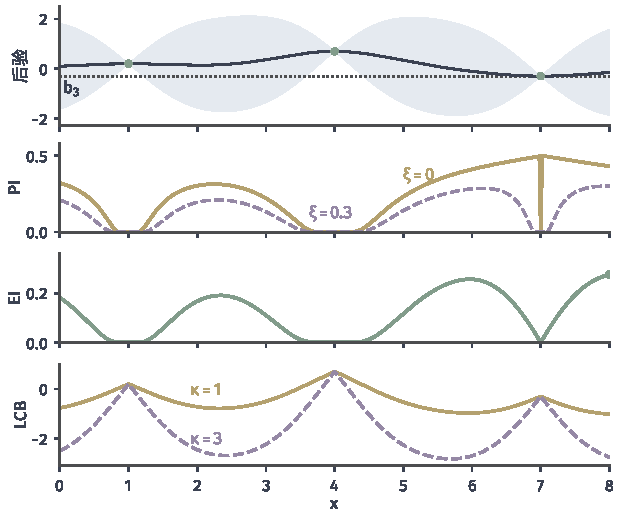
\includegraphics[width=105mm]{figures/05-optimization/05-stochastic-optimization/matplotlib/bo-acq-compare/figure.pdf}
 \caption{三种采集函数的比较，$t=3$，读数在$x=1,4,7$。第一行：深色线是后验均值，浅蓝带是均值上下两倍标准差，点线是$b_3$。第二行：改进概率，黄线$\xi=0$，紫虚线$\xi=0.3$。第三行：期望改进，绿点是最大点。第四行：置信下界，黄线$\kappa=1$，紫虚线$\kappa=3$，选点取最小点。}
 \label{fig:bo-acq-compare}
\end{BookInlineFigure}

\subsection{Thompson 采样}
\label{sec:bo-thompson}

前三种规则都把后验压缩成一个分数。\term{Thompson采样}（Thompson sampling）换了一种做法：不算分数，从当前后验抽取一整条函数$\widetilde{F}$，假装它就是真实目标，然后选它的最小点：
\begin{equation}
 \bm{x}_{t+1}\in\argmin_{\bm{x}\in\bm{C}}\widetilde{F}(\bm{x}),\qquad
 \widetilde{F}\sim F\mid\mathcal{D}_t.
 \label{eq:bo-thompson}
\end{equation}
一个位置被选中的概率，等于后验认为它是最小点的概率。乐观与谨慎不需要权重来调，而由后验分布本身决定：不确定的地方抽样起伏大，有机会被选中，但机会并不独占。

\paragraph{抽样要联合}
在有限候选集$\bm{x}_{1}',\ldots,\bm{x}_{N}'$上，抽样要从多元高斯分布$N(\bm{\mu},\bm{\Sigma})$抽取，$\bm{\mu}$和$\bm{\Sigma}$分别是后验均值向量和后验协方差矩阵。常用办法是作Cholesky分解$\bm{\Sigma}=\bm{L}\bm{L}^\top$，抽取标准正态向量$\bm{z}$，令
\begin{equation}
 \widetilde{\bm{F}}=\bm{\mu}+\bm{L}\bm{z}.
 \label{eq:bo-joint-sample}
\end{equation}

以$t=3$时的候选$x=6,8$为例。后验协方差矩阵和分解为
\[
 \bm{\Sigma}=\begin{bmatrix}0.746&-0.187\\-0.187&0.750\end{bmatrix},\qquad
 \bm{L}=\begin{bmatrix}0.864&0\\-0.217&0.838\end{bmatrix}.
\]
这里协方差是负的，这有一点反直觉：两点都与$x=7$相关，而$F(7)$已经确定，第~\ref{sec:bo-sequential}节会解释这个负号。

取$\bm{z}=(1,-0.5)^\top$，代入式~\eqref{eq:bo-joint-sample}，
\[
 \widetilde{F}(6)=-0.107+0.864=0.757,\quad
 \widetilde{F}(8)=-0.151-0.217-0.419=-0.787,
\]
这条样本的最小点在$x=8$。取$\bm{z}=(-1,0.5)^\top$，则
\[
 \widetilde{F}(6)=-0.971,\quad\widetilde{F}(8)=0.485,
\]
这条样本选$x=6$。两种结果都可能发生，选点因此带有随机性。

若把各点的边际分布独立抽样，得到的就不是后验函数。图~\ref{fig:bo-ts-paths}对比了在$0.1$网格上的两种抽样。(a)联合抽样是一条光滑曲线，穿过全部读数。(b)独立抽样忽略了相邻点的相关性，成了一串噪声，最小点总会落在方差最大的某处，这不是后验认为最可能的最小点。按20000条联合样本统计，最小点约四分之一的机会落在$x=8$附近，约四分之一的机会落在$x=6$附近，其余分散到$x=0$和$x=2$等位置。

\begin{BookInlineFigure}
 \centering
 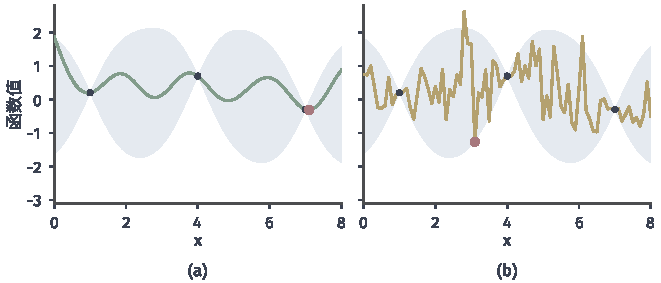
\includegraphics[width=112mm]{figures/05-optimization/05-stochastic-optimization/matplotlib/bo-ts-paths/figure.pdf}
 \caption{联合抽样与边际独立抽样。浅蓝带是$t=3$的后验均值上下两倍标准差，黑点是读数，红点是样本的最小点。(a)联合抽样得到的绿色曲线是一条可能的函数。(b)各网格点独立抽样得到的黄线不对应任何一条函数，把它的最小点当作选点并无依据。}
 \label{fig:bo-ts-paths}
\end{BookInlineFigure}

计算上，$N$个候选的联合抽样要作一次$O(N^3)$的分解。连续搜索域上不能抽取真正的无穷维函数，通常在较大的候选集上离散化，或用有限维随机特征近似，这些都是近似的来源。

\subsection{知识梯度（补充）}
\label{sec:bo-kg}

EI衡量的是“这次读数本身比现在最好的值低多少”。可是我们最终要交付的是推荐解，而一次读数即使本身不好，也可能让我们更清楚哪个位置该推荐。本小节换一个问题：这次观测能让最终推荐改善多少？

\paragraph{定义}
取一个推荐集合$\bm{R}\subseteq\bm{C}$，当前的最优推荐价值是后验均值的最小值$\min_{\bm{x}'\in\bm{R}}m_t(\bm{x}')$。设想在$\bm{x}$再观测一次，更新后的后验均值为$m_{t+1}$，它依赖尚未发生的读数，因而是随机的。\term{知识梯度}（knowledge gradient，KG）定义为
\begin{equation}
 \mathrm{KG}_t(\bm{x})=\min_{\bm{x}'\in\bm{R}}m_t(\bm{x}')-\mathbb{E}\Bigl[\min_{\bm{x}'\in\bm{R}}m_{t+1}(\bm{x}')\,\Bigm|\,\mathcal{D}_t,\bm{x}_{t+1}=\bm{x}\Bigr].
 \label{eq:bo-kg}
\end{equation}
更新后的均值以当前均值为期望，也就是
\[
 \mathbb{E}\bigl[m_{t+1}(\bm{x}')\mid\mathcal{D}_t\bigr]=m_t(\bm{x}').
\]
$\min$是凹函数，凹函数的期望不超过期望处的函数值（Jensen不等式），所以$\mathrm{KG}_t(\bm{x})\geq0$。

下一次读数的预测分布是$N(m_t(\bm{x}),s_t^2(\bm{x})+\tau^2)$，把标准化的预测残差记作$Z\sim N(0,1)$。把定理~\ref{thm:bo-posterior}应用于“以当前后验为先验、只含这一个观测”的情形，可得
\begin{equation}
 m_{t+1}(\bm{x}')=m_t(\bm{x}')+\widetilde{\sigma}_t(\bm{x}',\bm{x})Z,\quad
 \widetilde{\sigma}_t(\bm{x}',\bm{x})=\frac{c_t(\bm{x}',\bm{x})}{\sqrt{s_t^2(\bm{x})+\tau^2}}.
 \label{eq:bo-kg-update}
\end{equation}
每个推荐点的后验均值都随同一个$Z$线性移动，斜率取决于它与被观测位置的后验协方差。式~\eqref{eq:bo-kg}中的期望因此是一维积分，有限的$\bm{R}$上可以用分段线性包络精确算出，也可以用数值积分。

\paragraph{例：观测一个不推荐的位置}
取$\bm{R}=\{6,7\}$，当前后验均值$m_3(6)=-0.107$，$m_3(7)=-0.3$，当前最优推荐是$x=7$，价值$-0.3$。考虑观测$x=5$，它本身不在$\bm{R}$里。$x=7$已观测，$c_3(7,5)=0$，均值不动。由$c_3(6,5)\approx0.438$和$s_3(5)\approx0.864$，
\[
 \widetilde{\sigma}_3(6,5)\approx\frac{0.438}{0.864}\approx0.507.
\]

新的最优推荐价值是$\min\{-0.3,\ -0.107+0.507Z\}$。这个最小值可以写成$-0.3$减去$-0.3$与第二项之差的正部，代入式~\eqref{eq:bo-kg}，$\mathrm{KG}$恰好是阈值为$-0.3$的EI公式，只是均值和标准差换成$-0.107$与$0.507$：
\[
 \mathrm{KG}_3(5)\approx(-0.193)\Phi(-0.381)+0.507\,\phi(-0.381)\approx0.120.
\]
这个$x=5$的读数本身比$-0.3$低的可能性不大，因而$\mathrm{EI}_3(5)\approx0.117$，它的价值主要来自让我们更好地判断$x=6$。此处的KG同样不要求评价点属于$\bm{R}$，这是它与EI的不同，也允许最后推荐一个未曾评价的位置。

图~\ref{fig:bo-kg-vs-ei}比较了EI和取$\bm{R}$为$0.1$网格时的KG。两者的形状相近，但KG的最大点在$x\approx7.1$，紧靠当前最好点。在无噪声且核很光滑的模型中，贴着已知点再读一次，相当于测得该处的斜率，它能改变整段后验均值的最小位置，所以KG偏爱这里；而在恰好已观测的点上，读数不带来任何新信息，KG降为$0$，图中出现几个尖口。

\begin{BookInlineFigure}
 \centering
 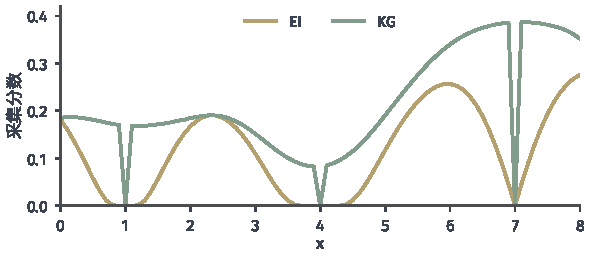
\includegraphics[width=100mm]{figures/05-optimization/05-stochastic-optimization/matplotlib/bo-kg-vs-ei/figure.pdf}
 \caption{EI与KG的对比，$t=3$，无噪声观测。黄线是期望改进，绿线是知识梯度（推荐集合为$0.1$网格，期望由$401$个等分位点数值积分）。KG在已观测点$x=1,4,7$上为$0$，在紧邻这些点的位置却不为$0$。}
 \label{fig:bo-kg-vs-ei}
\end{BookInlineFigure}

KG的计算比EI贵，并且对模型更敏感。一般的实验设计问题以信息价值安排观测，可参考\BookChapterRef{chap:observation-experiment-design}{卷八第9章“观测与实验设计”}；本章只把KG作为一种选点规则，在第~\ref{sec:bo-noisy}节有噪声时会再次用到它。
